%%%%%%%%%%%%%%%%%%%%%%%%%%%%%%%%%%%%%%%%%%%%%%%%%%%%%%%%%%%%%%%%%%%%%%%%%
%%%%%%%%%%%%%%%%%%%%%%%%%%%%%%%%%%%%%%%%%%%%%%%%%%%%%%%%%%%%%%%%%%%%%%%%%
%%%%%%%%%%%%%%%%%%%%%%%%%%%%%%%%%%%%%%%%%%%%%%%%%%%%%%%%%%%%%%%%%%%%%%%%%
\section{$BV^2$-piecewise Similarity Motions}\label{similarity}

In order to improve the matching results we augment our model by allowing the curve to shrink or to lengthen during the evolution. The idea consists in considering evolution by piecewise similarity motions instead of the rigid deformations considered in Section~\ref{PWR}.  

%%%%%%%%%%%%%%%%%%%%%%%%%%%%%%%%%%%%%%%%%%%%%%%%%%%%%%%%%%%%%%%%%%%%%%%%%
\subsection{Similarity Curve Deformations}

We extend the rigid deformations considered in Section~\ref{GRD} to smooth evolutions $t \mapsto \Ga_t$ following a PDE~\eqref{eq-continuous-flow} that includes also a global scaling of the space. This evolution is said to obey a similarity transform if there exists a smooth function $\la : \RR \rightarrow \RR^+$ such that
\eql{\label{eq-similarity-flow}
	\foralls (s,s') \in \Circ \times \Circ, \quad
	\norm{\GA_t(s)-\GA_t(s')} = \la(t) \norm{\GA_0(s)-\GA_0(s')}.
} 
The following proposition states that the set of instantaneous motions $\Phi_t$ giving rise to a similarity evolution  is, at each time, a linear sub-space of dimension 4 of $T_{\Ga_t} \Bb$.

\begin{prop}
	The evolution~\eqref{eq-continuous-flow} satisfies~\eqref{eq-similarity-flow} if and only if, for all $t \in \RR$, $\Phi_t \in \Ss_{\GA_t}$ where  
	\eql{\label{eq:similarity}
		\Ss_\GA = \enscond{ \Phi \in T_\Ga \Bb }{
			\foralls s \in \Circ, \; \Phi(s) =  A \GA(s)  +  b:
			\;\text{for}\; 
			A \in \Ss_{2 \times 2}, \: b \in \R^2
		}
	}
	\eq{
		\qwhereq
		\Ss_{2 \times 2} = \enscond{
		\begin{pmatrix}
					\al& -\be\\
					\be&\al\\
			\end{pmatrix} \in \RR^{2 \times 2}
		}
		{ (\al,\be) \in \RR^2 }
	\,.}
\end{prop}
\begin{proof}
Using the fact that the Lie algebra of the group of similarities is $\R^2 \rtimes \Ss_{2 \times 2}$, we obtain the desired result following the proof of Proposition \ref{rigid-ch}. %Note that the scaling parameter can be fixed using the surface defined by the three points.
%\textcolor{red}{donner argument groupes de lie}
%By the definition of evolution, we have\begin{equation}\label{second-rigid}\GA_t(s)= \GA_0(s)+ \int_0^t \Phi_{\tau}(s)\d \tau \quad \forall s\in \Circ\,,\end{equation}If the evolution verifies~\eqref{eq-similarity-flow}, the previous relationship defines a similarity transformation between $\GA_0(\Circ)$ and $\GA_t(\Circ)$. By the same argument used in the proof of Proposition~\ref{rigid-ch}, such a transformation can be extended to a similarity transformation of the plane. Then, by the characterization of the similarity transformations of the plane,  we get that\begin{equation}\label{first-rigid}\GA_t(s)= S(t)\GA_0(s) + c(t)\quad \forall s\in \Circ\end{equation}for some vector $c(t)$ and  matrix $S(t)\in \Ss_{2 \times 2}$ $$S(t)=\begin{pmatrix}				\al(t)& -\be(t)\\					\be(t)&\al(t)\\\end{pmatrix}\,.$$Now, by differentiating~\eqref{second-rigid} and~\eqref{first-rigid}   with respect to $t$,we get\begin{equation}\label{third-rigid}\Phi_t(s)= S'(t)\GA_0(s) + c'(t) \quad \forall s\in \Circ\end{equation}where $(\cdot)'$ denotes here the derivation with respect to $t$. Then by~\eqref{first-rigid} and~\eqref{third-rigid} we get $$\Phi_t(s)= S'(t)S(t)^{-1}\GA_t(s) + c'(t)- S'(t)S(t)^{-1}c(t) \quad \forall s\in \Circ\,$$which implies that $\Phi_t \in \Ss_{\GA_t}$ with $A=S'(t)S(t)^{-1}\in \Ss_{2 \times 2}$ and $b=c'(t)- S'(t)S(t)^{-1}c(t)$.\par Conversely, if $\Phi_t \in \Ss_{\GA_t}$,  we have  $$(\Phi_t(s)-\Phi_t(s'))\cdot(\GA_t(s)-\GA_t(s')) =\alpha(t)\norm{\GA_t(s)-\GA_t(s')}^2\,,\quad \foralls (s,s') \in \Circ \times \Circ\,$$for some $\al(t)\in \R$. This means that $$\frac{\partial}{\partial t} \norm{\GA_t(s)-\GA_t(s')}^2 = \frac{\alpha(t)}{2} \norm{\GA_t(s)-\GA_t(s')}^2\,,\quad \foralls (s,s') \in \Circ \times \Circ$$which implies that$$ \norm{\GA_t(s)-\GA_t(s')}^2 = e^{\int_0^t\al(\tau)/2\d \tau} \norm{\GA_0(s)-\GA_0(s')}^2\,,\quad \foralls (s,s') \in \Circ \times \Circ$$and this proves that the $\Phi_t$ verifies~\eqref{eq-similarity-flow} with $\lambda(t)= e^{\int_0^t\al(\tau)/2\d \tau}$.
\end{proof}

Analogously to Proposition~\ref{charactrigid}, the next proposition characterizes in an intrinsic manner the set~$\Ss_\Ga$.

\begin{prop}\label{similitude}
	For a $C^2$-curve $\Ga$, one has $\Phi \in \Ss_\GA$ if and only if $\Phi$ is $C^2$ and satisfies 
\begin{equation}\label{similarity0}
		\frac{\d K_\GA(\Phi)}{\dgs} = 0
		\end{equation}
	where we have introduced the following linear operator 
	\eq{	
		K_\GA(\Phi)=\left(\frac{\d \Phi}{\d \GA}\cdot \tgam, \frac{\d \Phi}{\d \GA}\cdot \ngam \right), 
		\quad \quad\foralls \Phi \in T_\GA\Bb\,.
	}
\end{prop}

\begin{proof}
Given a curve $\GA\in C^2(\Circ,\RR^2)$, every   deformation $\Phi$ of $\Gamma$ which is the restriction, to the curve $\Gamma$,  of an instantaneous similarity motion, can be written as
\eq{
	\Phi(s) \; = \;  A \GA(s)  + b, \quad \quad \foralls s\in \Circ 
}
for some matrix $A=\begin{pmatrix}
\al& -\be\\
\be&\al\\
\end{pmatrix} $ and a vector $b$.
Now, differentiating with respect to $\d \GA$ we obtain
\eq{
	\frac{\d\Phi}{\dgs}(s)= A\tgam
}
which is equivalent to  
\begin{equation}\label{similarity-eqz}
	\frac{\d \Phi}{\dgs}  \cdot\, \tgam \; = \; 
	 \alpha 
	\qandq
	\frac{\d \Phi}{\dgs}  \cdot\, \ngam \; = \; 
	 \beta
\end{equation}
for every $s\in \Circ$. Remark that similarity  is the only affine motion verifying~\eqref{similarity-eqz} and this is due to the form of the matrix $A$. In fact, if $\frac{\d \Phi}{\dgs} $ verifies $\frac{\d \Phi}{\dgs}  \cdot\, \tgam = \alpha$ and $\frac{\d \Phi}{\dgs}  \cdot\, \ngam= \beta$ then
$$\frac{\d \Phi}{\dgs} = \alpha \tgam + \beta \ngam = \alpha \tgam + \beta \tgam^\bot = A\tgam\,.$$ 
In particular, if $\alpha = 0$ then $\Phi$ is a rigid motion and~\eqref{similarity-eqz} coincides with the characterization proved in Proposition~\ref{charactrigid}.

Then, differentiating again with respect to $d \GA(s)$, we have
\eq{
	\frac{\d}{\dgs}\left(\frac{\d \Phi}{\dgs}  \cdot\, \tgam\right) \; = \; 0
	\qandq
	\frac{\d}{\dgs}\left(\frac{\d \Phi}{\dgs}  \cdot\, \ngam\right) \; = \; 0
}
which is equivalent to~\eqref{similarity0}.
\end{proof}

%%%%%%%%%%%%%%%%%%%%%%%%%%%%%%%%%%%%%%%%%%%%%%%%%%%%%%%%%%%%%%%%%%%%%%%%%%%%
\subsection{Piecewise Similarity Deformations}


Similarly to the Finsler penalty introduced in~\ref{BV2M}, we define a penalty that favors piecewise similarity transformations  by minimizing  the $L^1$-norm of the first derivative of $K_\GA$. To control the piecewise rigid transformation part, we relax the equality constraint $L_\GA(\Phi)=0$ defined as $\Cc_\Ga$ in~\eqref{eq-constr-C-Ga} to  a constraint $\Cc_\Ga^\la$ on the $L^1$ norm of $L_\GA(\Phi)$. 


\begin{defn}[\BoxTitle{Piecewise-similarity penalty}]\label{defn2} For $\la \geq 0$ and $\Ga \in \Bb$, we define for all $\Phi \in T_\Ga\Bb$
\begin{equation}\label{eq-piecewise-similarity-penalty}
	R_\Ga^\la(\Phi) =
	TV_\GA(K_\GA(\Phi) )
	+ \iota_{\Cc_\Ga^\la}
	\qwhereq
	\Cc_\Ga^\la = \enscond{ \Phi \in T_\GA \Bb }{
			\norm{L_\Ga(\Phi)}_{L^1(\Ga)}\leq \la }
\end{equation}
where $L_\Ga$ is either $L_\Ga^+$ or $L_\Ga^-$ as defined in~\eqref{eq-operator-L} and $TV_\GA$ is defined in~\eqref{TV}.
\end{defn}


The piecewise similarity Finsler gradient $\nabla_{R_\Ga^\la}E(\Ga)$ is defined by minimizing~\eqref{defgrad} with the penalty $R_\Ga^\la$ defined in~\eqref{eq-piecewise-similarity-penalty} with the constraint set $\Ll_\Ga$ defined in~\eqref{eq-dev-constr}.  The following proposition shows that, as $\la$ tends to 0, the set of piecewise similarity Finsler gradients tends to the set of piecewise-rigid Finsler gradients. 

\begin{prop}
	One has $R_\Ga^0 = R_\Ga$ where $R_\Ga$ is defined in~\eqref{eq-piecewise-rigid-penalty}.
\end{prop}
\begin{proof}
One has $\Cc^0_\Ga = \Cc_\Ga$.
If $R_\Ga^0(\Phi) \neq +\infty$, one has $L_\GA^{+}(\Phi)=L_\GA^{-}(\Phi)=0$ a.e., so that in this case 
\eq{
	TV_\GA( K_\Ga(\Phi) )= 
	TV_\GA\left(\frac{\d \Phi}{\d \GA(s)}\cdot \ngam \right)\,.}
\end{proof}
The following theorem extends Theorem~\ref{existence1} to the piecewise similarity penalty and ensures existence of the corresponding Finsler gradient.

 
\begin{thm} 
The function $R_\GA^\la$ defined in~\eqref{eq-piecewise-similarity-penalty} admits at least a minimum on $\Ll_\GA$. 
\end{thm}

\begin{proof} 
	It suffices to adapt the proof of Theorem~\ref{existence1} by  using the new constraint on the $L^1$-norm of $L_\Ga(\Phi)$.
\begin{comment}
In fact as $\Phi'\cdot \tgam $ is bounded in $L^1$ its integral on $[s_0,s]$ is bounded $L^\infty$. Then  if~\eqref{writing-phi} contains a term depending on the tangential part of $\Phi'$, as it is bounded, we can prove~\eqref{bound-first-der}. Now, we can rewrite~\eqref{writing-phi} using the decomposition of $\Phi'\cdot \tgam= u+ a$ and taking the tangential projection. So we get that $\Phi(s_0)+a[\GA(s)-\GA(s_0)]\in \L^\infty$. By the same argument we prove that $\Phi'\cdot\tgam$ is bounded in $L^\infty$. Of course the bounds depend on $\lambda$. The end of the proof is the same.
\end{comment}

\end{proof}


%%%%%%%%%%%%%%%%%%%%%%%%%%%%%%%%%%%%%%%%%%%%%%%%%%%%%%%%%%%%%%%%%%%%
%%%%%%%%%%%%%%%%%%%%%%%%%%%%%%%%%%%%%%%%%%%%%%%%%%%%%%%%%%%%%%%%%%%%
%%%%%%%%%%%%%%%%%%%%%%%%%%%%%%%%%%%%%%%%%%%%%%%%%%%%%%%%%%%%%%%%%%%%
\subsection{Numerical examples}\label{NE}


We now show some numerical examples for the piecewise similarity Finsler gradient. The computation is performed with the discretization detailed in Section~\eqref{discretization}, which is extended in a straightforward manner to handle the piecewise similarity model.

\begin{figure}[!h]
\centering
\begin{tabular}{@{}c@{\hspace{5mm}}c@{}}
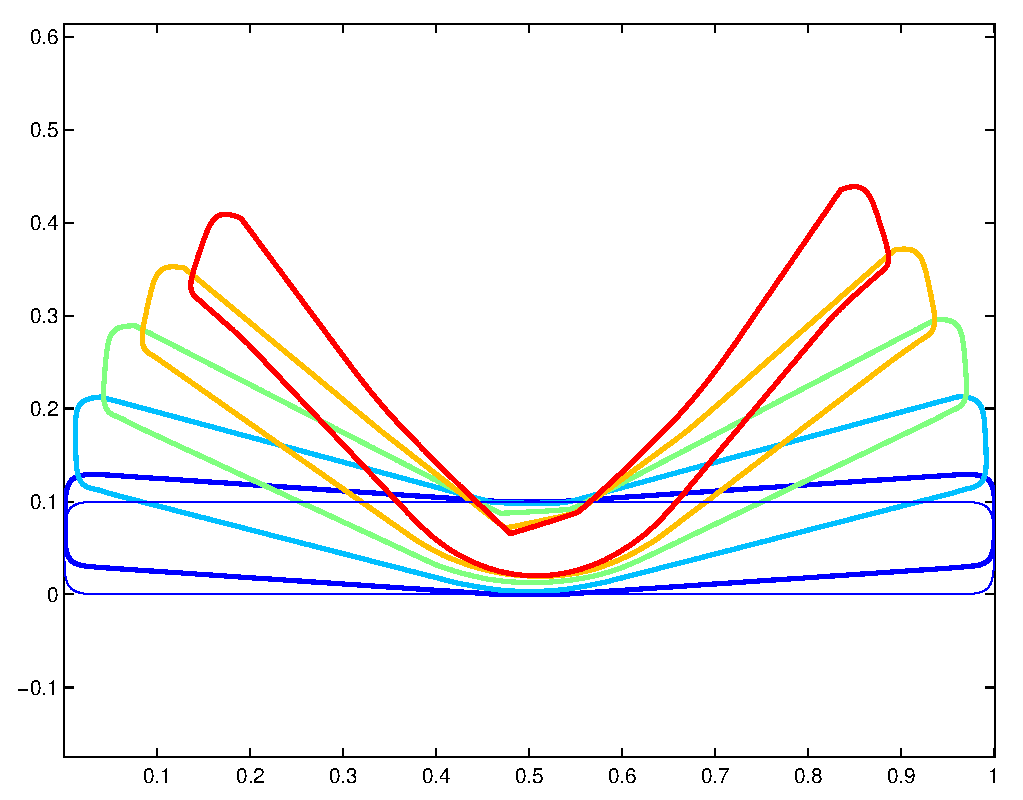
\includegraphics[width=.3\linewidth]{rod1-lambda}&
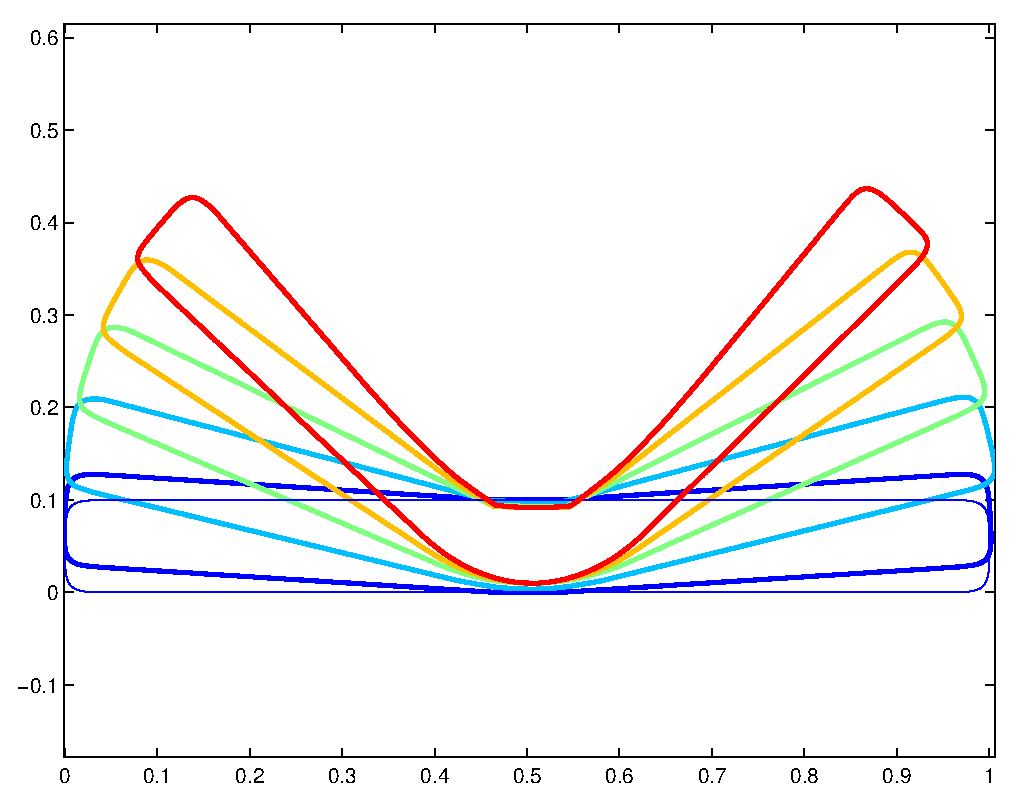
\includegraphics[width=.3\linewidth]{rod2-lambda}\\
$\la=.01$ & $\la=50$ \\
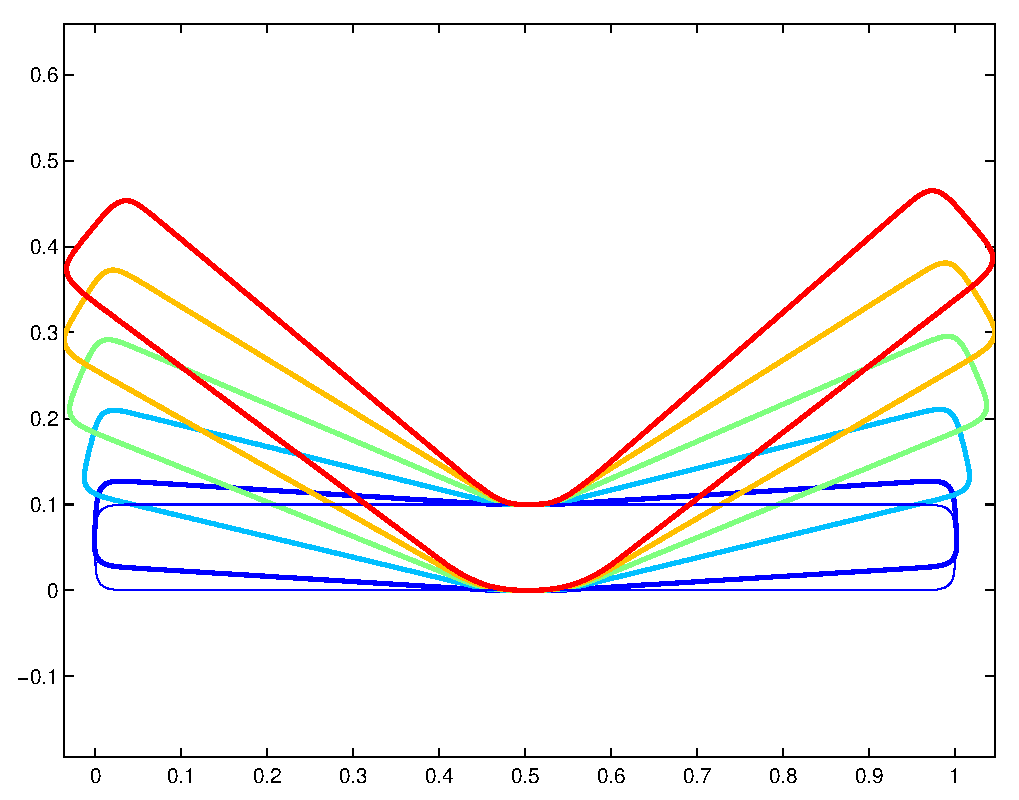
\includegraphics[width=.3\linewidth]{rod3-lambda}&
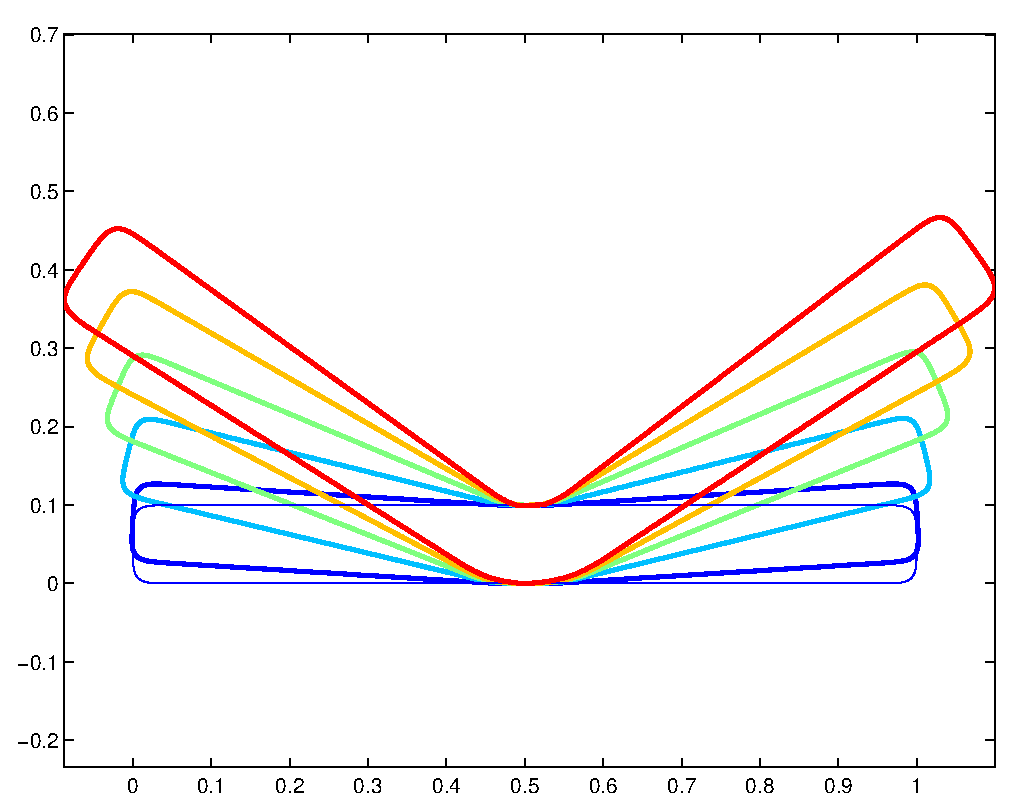
\includegraphics[width=.3\linewidth]{rod4-lambda}\\
 $\la=300$ & $\la=2000$
\end{tabular}
\caption{ Piecewise similarity Finsler flow evolutions for $\rho = 0.3$ and for different values of $\la$. }\label{evolutions2}
\end{figure}

%%%
\paragraph{Influence of  $\la$. }

We first re-use the synthetic example introduced in Section~\ref{sec-influ-rho} to illustrate the influence of the parameter $\la$. We thus use an evolution driven by the flow $F(\Ga) \in T_\Ga \Bb$ defined in~\eqref{field-const}. Figure~\ref{evolutions2} shows how $\la$ allows one to interpolate between the piecewise rigid model (when $\la=0$) to a piecewise similarity model when $\la$ increases.  For large value of $\la$, one clearly sees the global scaling introduced by the model which is helpful to better follow the flow of $F$. 


Figure~\ref{evolutions3} compares the evolution obtained with the initial flow~\eqref{eq-synthetic-flow} (corresponding to $(\rho,\la)=(0,0)$, i.e. the Finsler gradient is equal to $F(\Ga)$), the piecewise rigid flow (corresponding to $\rho>0$ and $\la=0$) and the piecewise similarity flow (corresponding to $\rho>0$ and $\la>0$).
 
\begin{figure}[!h]
\centering
\begin{tabular}{@{}c@{\hspace{3mm}}c@{\hspace{3mm}}c@{}}
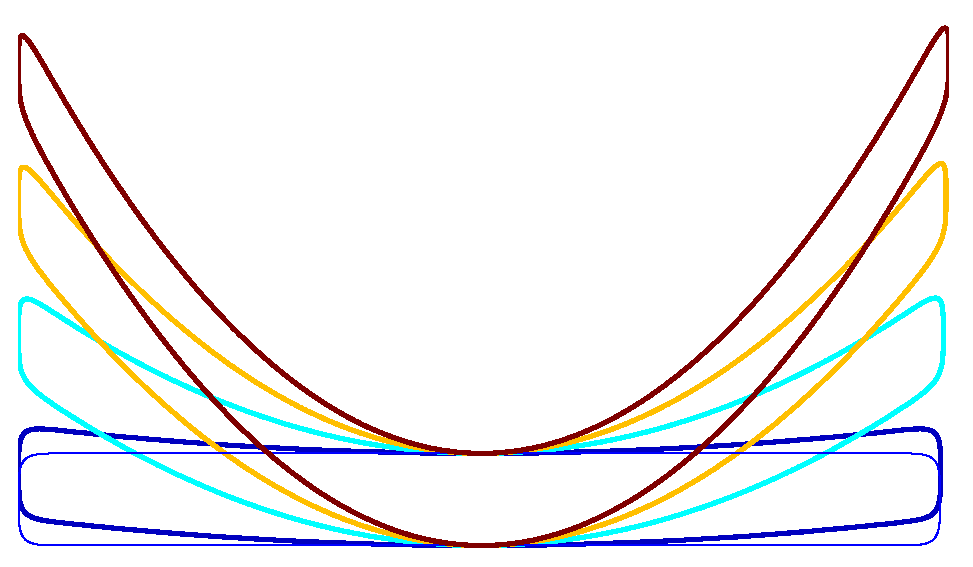
\includegraphics[width=.25\linewidth]{rod-L2}&
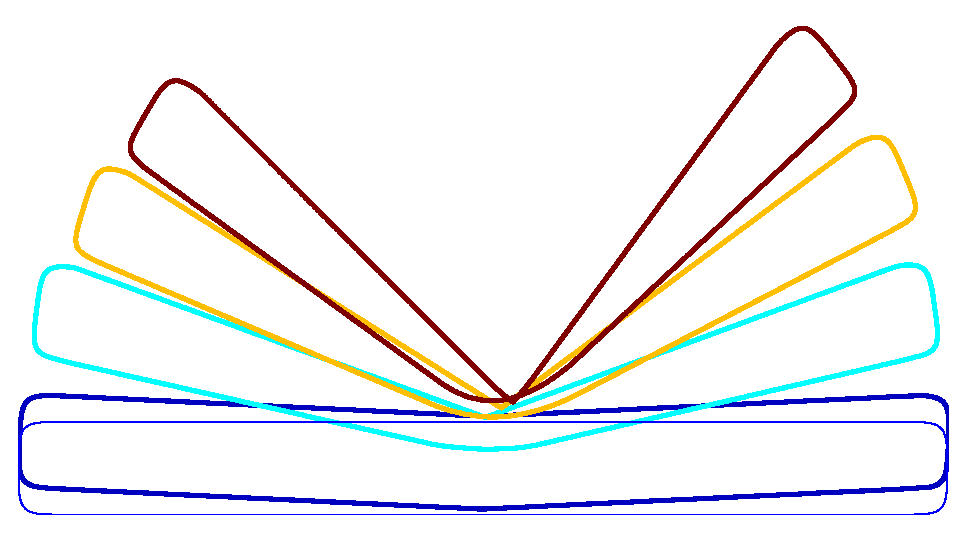
\includegraphics[width=.25\linewidth]{rod-Finsler1}&
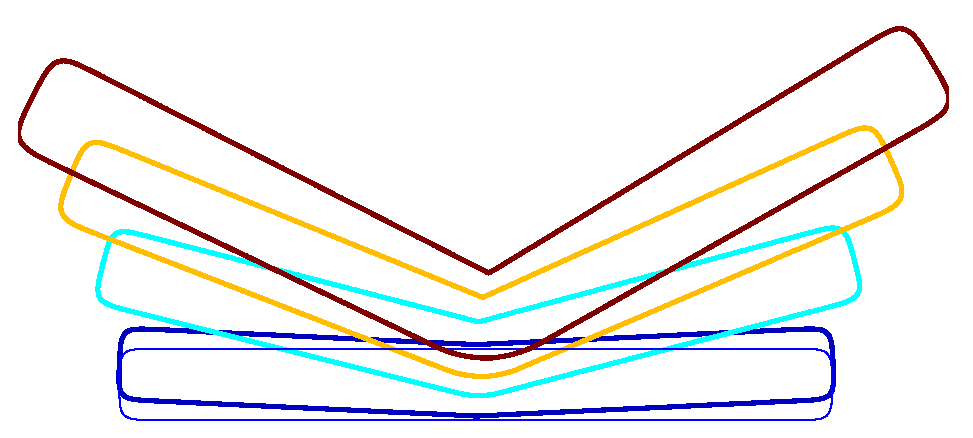
\includegraphics[width=.33\linewidth]{rod-Finsler2} \\
$L^2$ & $(\rho,\la)=(0.5,0)$ & $(\rho,\la)=(0.5,200)$ 
\end{tabular}
\caption{From left to right: evolutions by using the $L^2$ gradient, piecewise rigid Finsler gradient, piecewise similarity Finsler gradient. }\label{evolutions3}
\end{figure}

%%%
\paragraph{Application to the matching problem.}
 
We now show an application of the Finsler descent method to the curve matching problem, by minimizing the energy $E$ defined in~\eqref{energy}. Figure~\ref{evolutions} shows the results obtained with the piecewise similarity penalty for well chosen parameters $(\si,\de,\la,\rho)$. These evolutions should be compared with the ones reported in Section~\ref{sec-numerics-registration}. Allowing the length of the curve to vary using a parameter $\la>0$ allows the evolutions to better capture the geometry of the target shape and thus leads to better matchings. 

 
\begin{figure}[h]
\centering
\begin{tabular}{@{}c@{\hspace{1mm}}c@{\hspace{1mm}}c@{\hspace{1mm}}c@{\hspace{1mm}}c@{}}
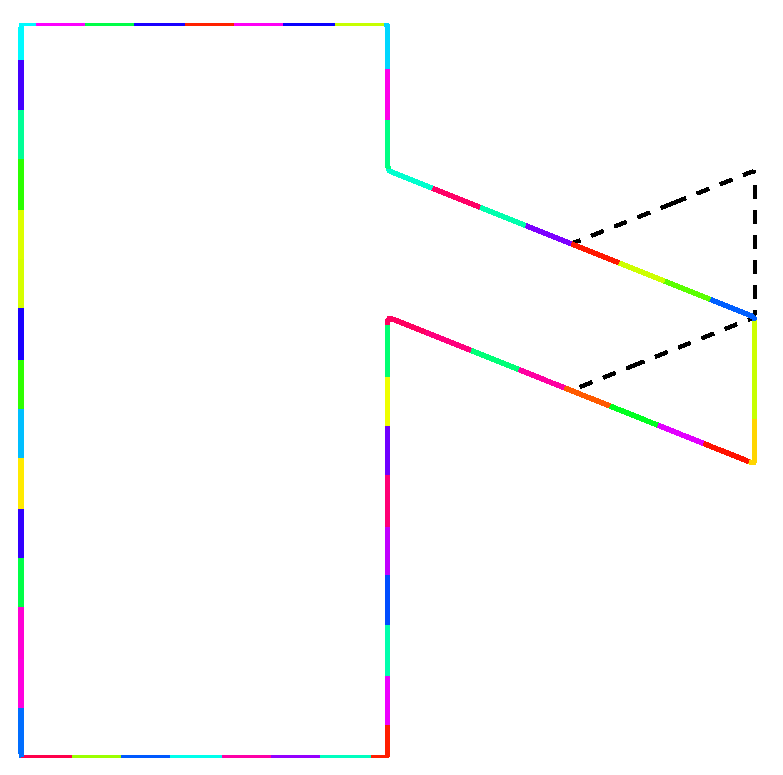
\includegraphics[width=.19\linewidth]{harm-finsler-simil--initial}&
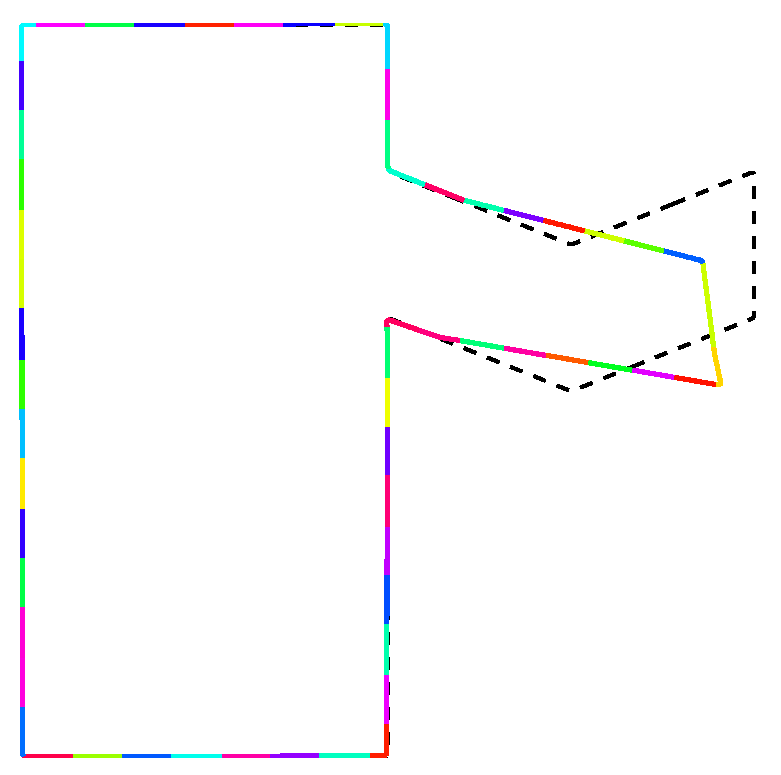
\includegraphics[width=.19\linewidth]{harm-finsler-simil-1}&
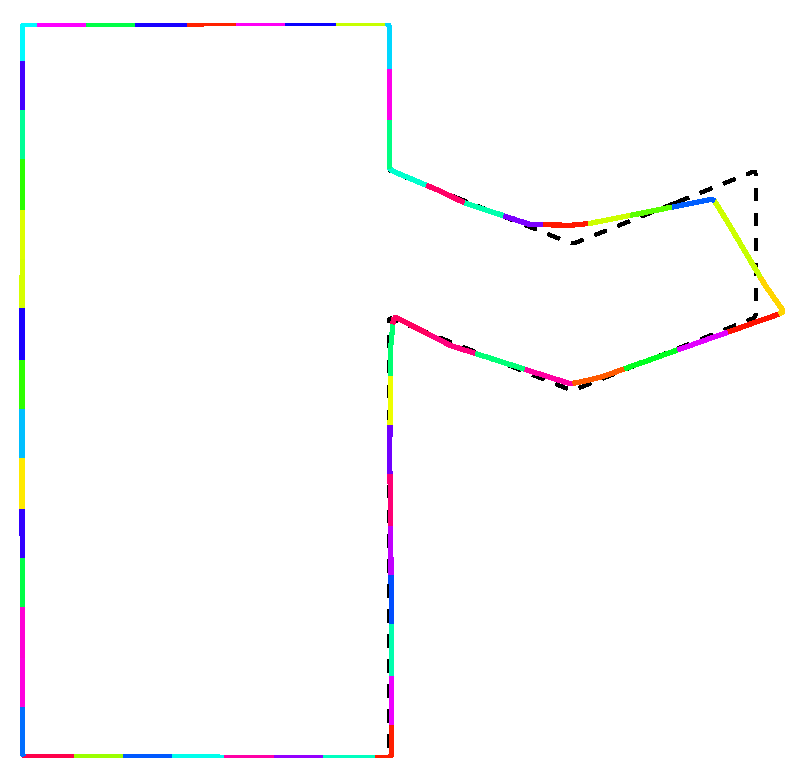
\includegraphics[width=.19\linewidth]{harm-finsler-simil-5}&
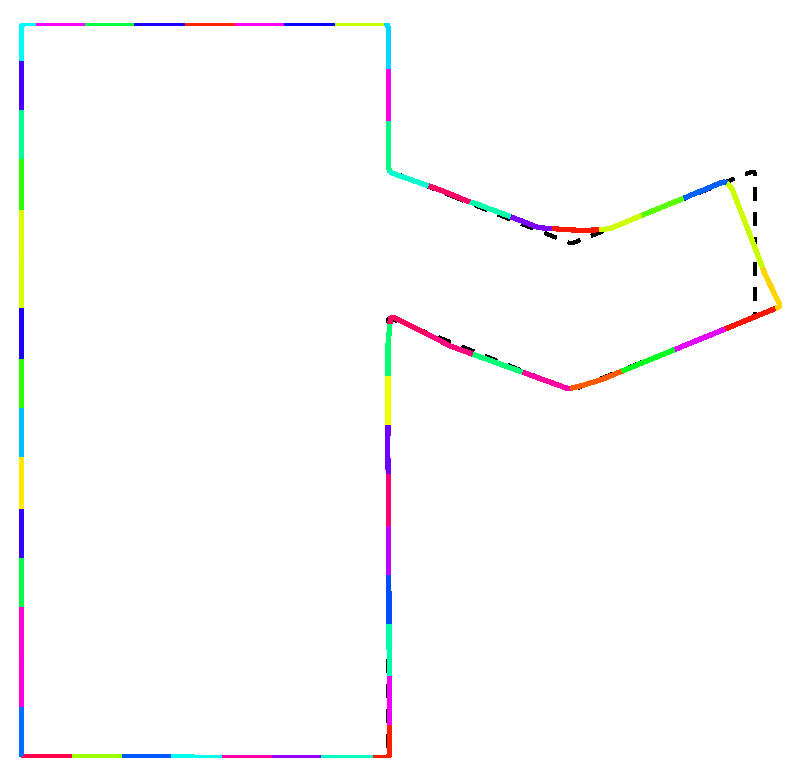
\includegraphics[width=.19\linewidth]{harm-finsler-simil-8}&
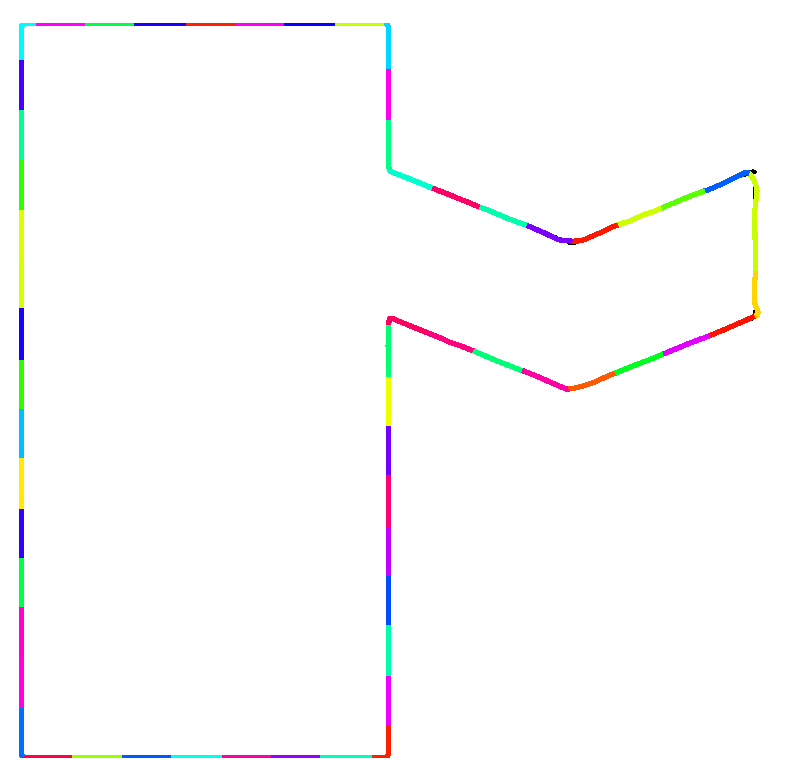
\includegraphics[width=.19\linewidth]{harm-finsler-simil--final}\\
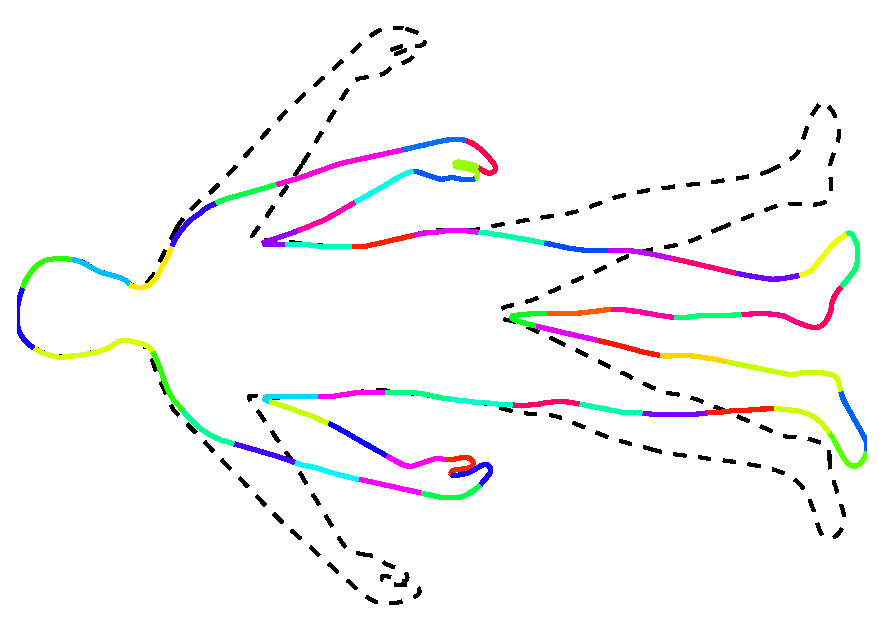
\includegraphics[height=.19\linewidth,angle=270]{man-finsler-simil--initial}&
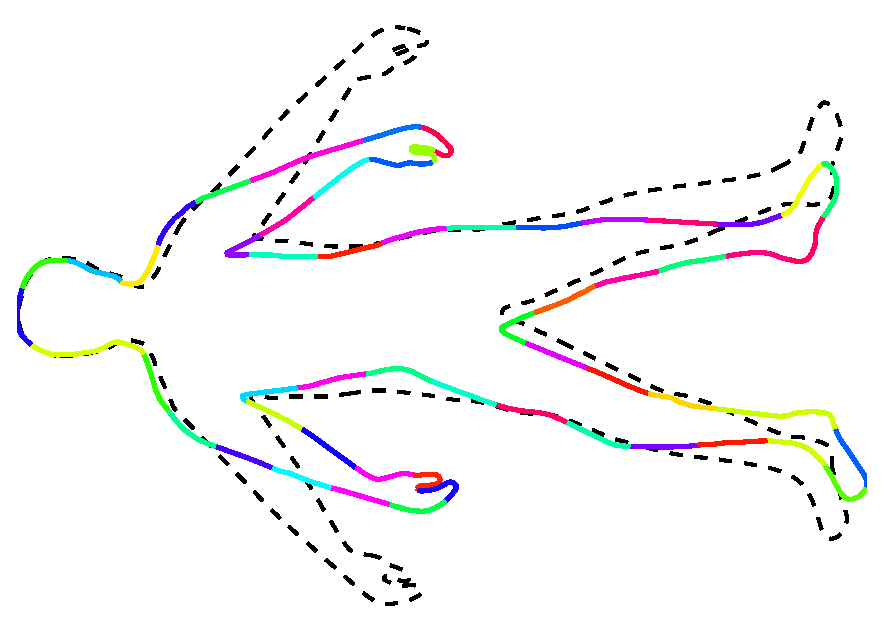
\includegraphics[height=.19\linewidth,angle=270]{man-finsler-simil-3}&
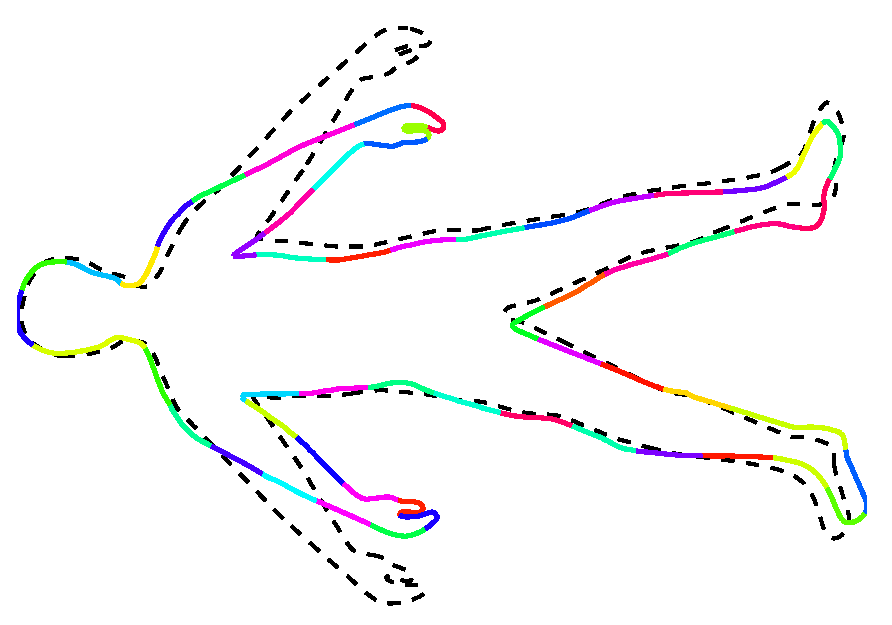
\includegraphics[height=.19\linewidth,angle=270]{man-finsler-simil-6}&
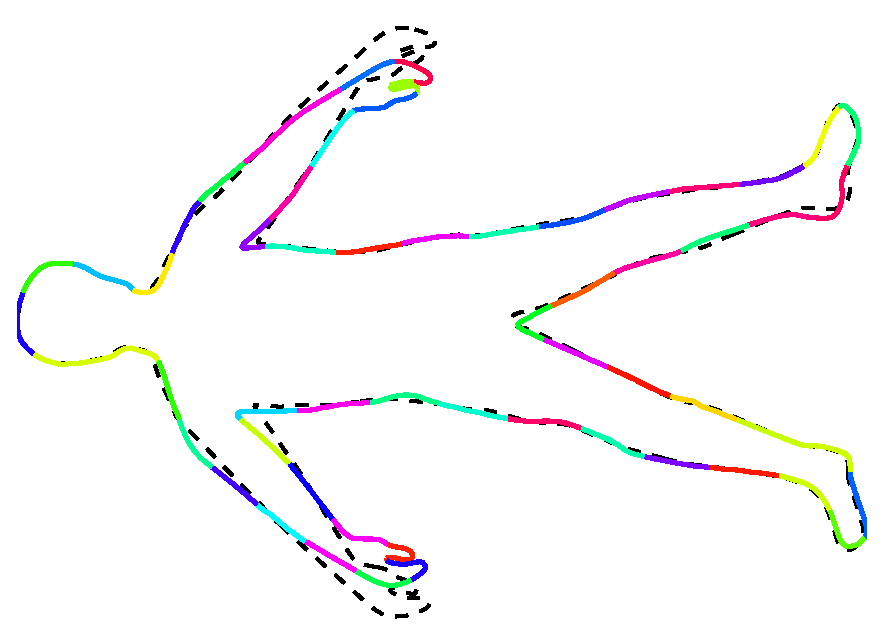
\includegraphics[height=.19\linewidth,angle=270]{man-finsler-simil-18}&
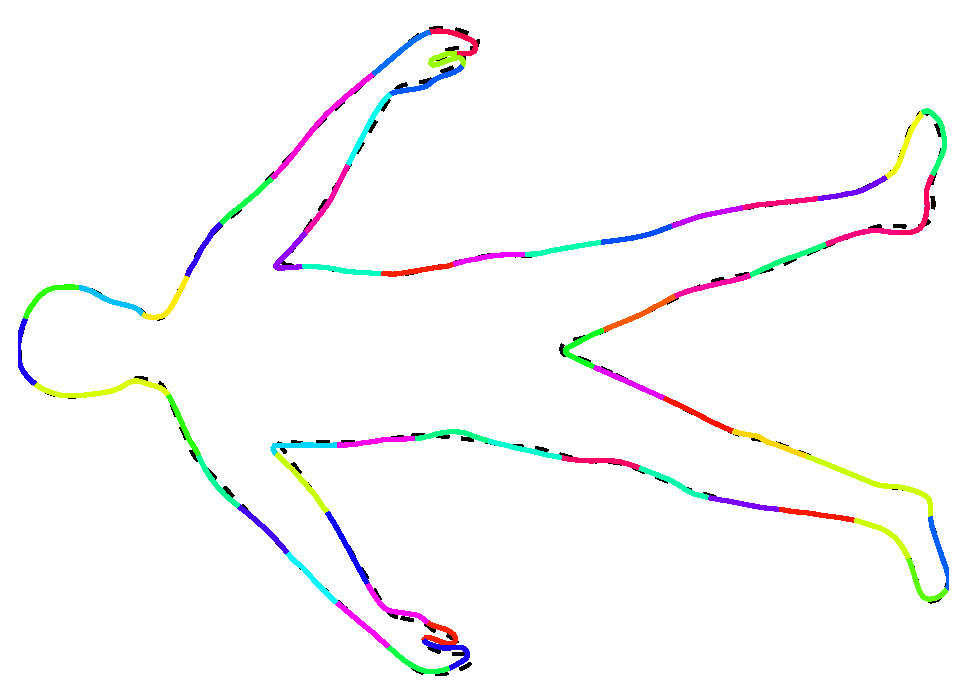
\includegraphics[height=.19\linewidth,angle=270]{man-finsler-simil--final}\\
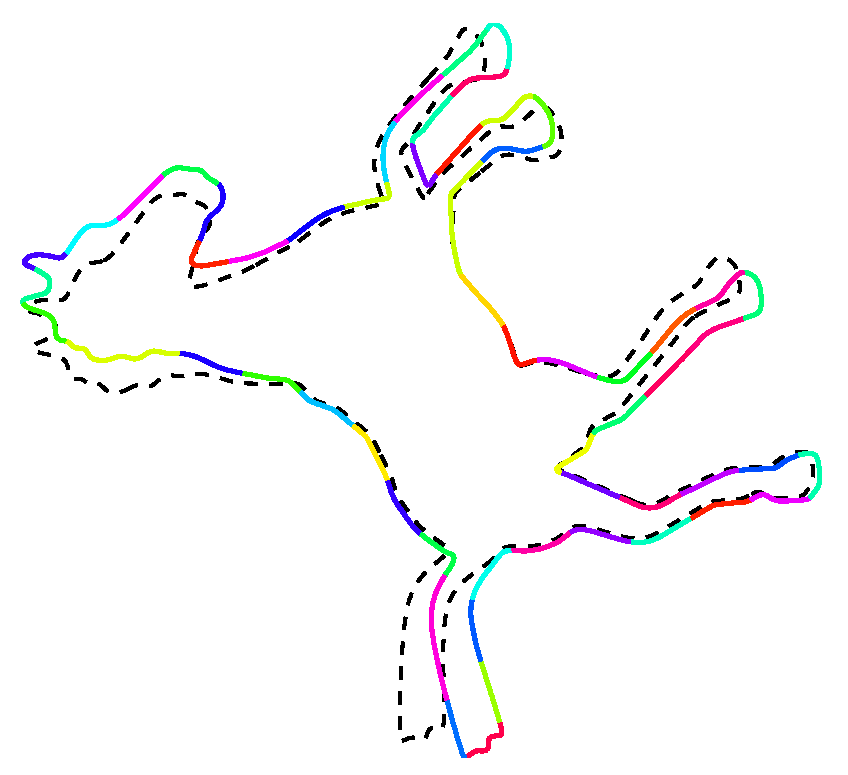
\includegraphics[height=.19\linewidth,angle=270]{horse-finsler-simil--initial}&
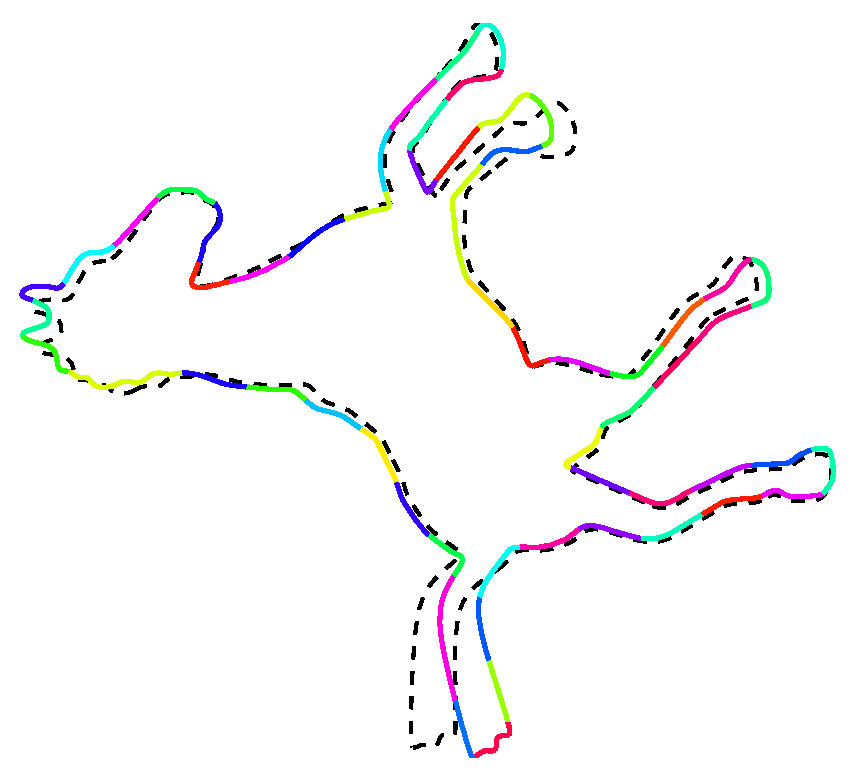
\includegraphics[height=.19\linewidth,angle=270]{horse-finsler-simil-1}&
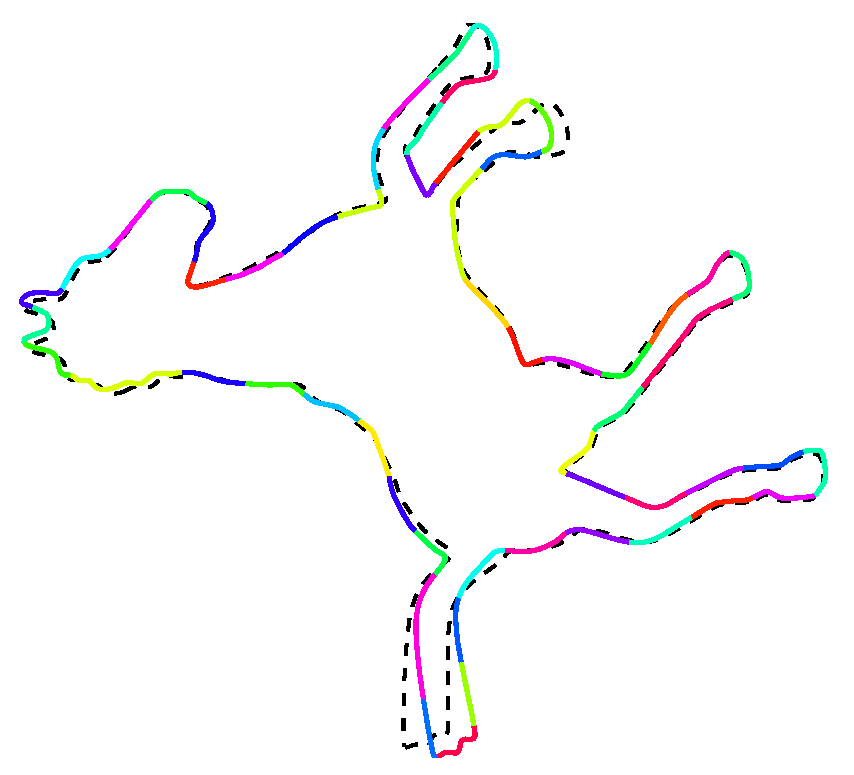
\includegraphics[height=.19\linewidth,angle=270]{horse-finsler-simil-3}&
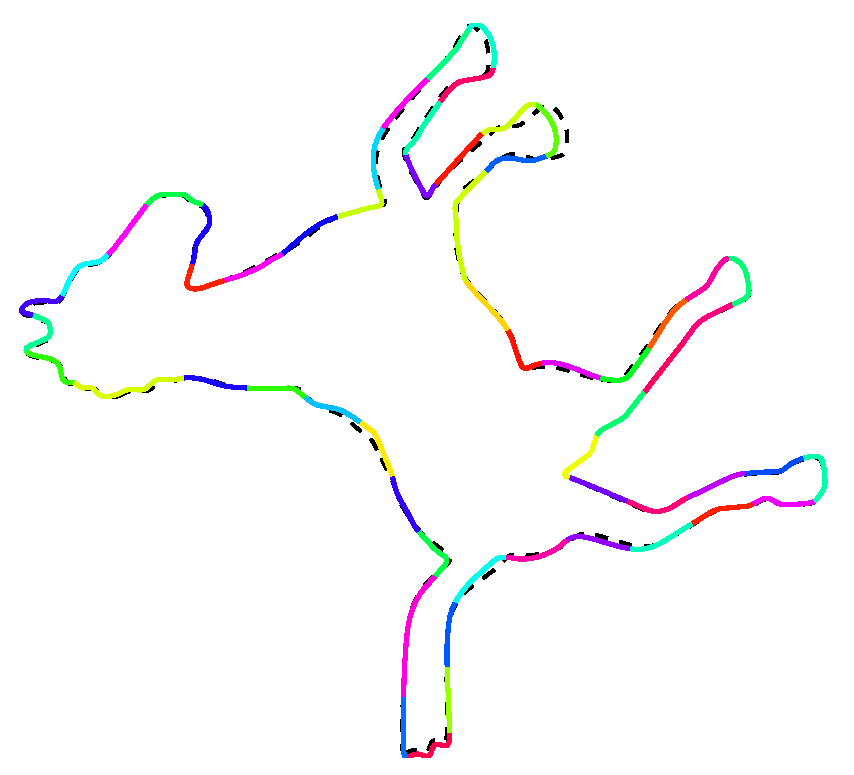
\includegraphics[height=.19\linewidth,angle=270]{horse-finsler-simil-5}&
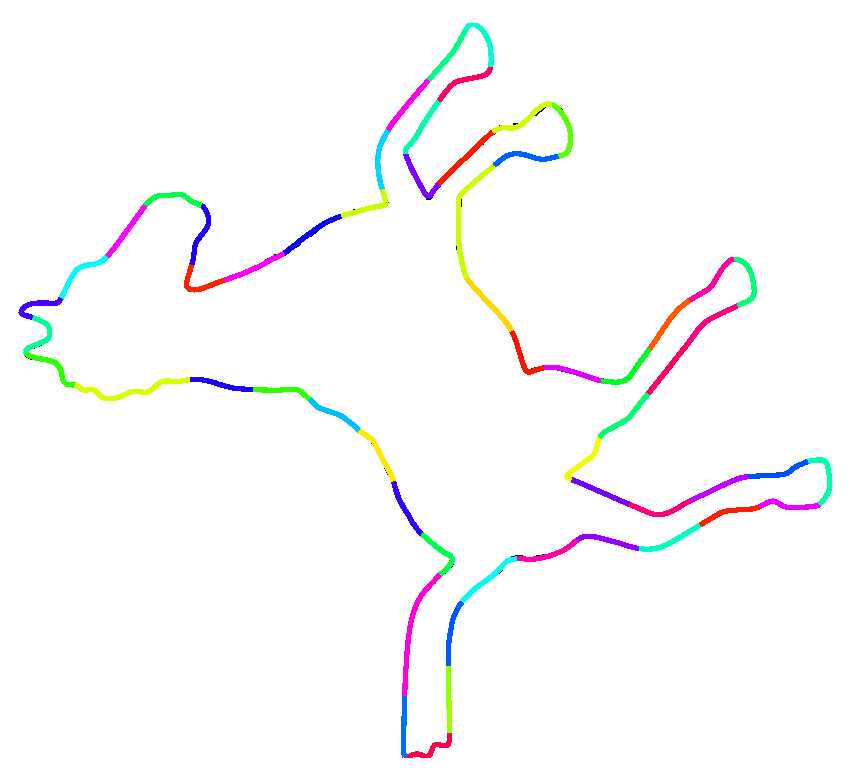
\includegraphics[height=.19\linewidth,angle=270]{horse-finsler-simil--final}
\end{tabular}
\caption{\label{evolutions} Curve matching by piecewise similarity motions. Each image displays the target curve $\La$ (dash line) and the current curve $\Ga_k$ (solid line). We used the following parameters: 
	top row: $\sigma=0.8$, $\delta=0.04$, $\la=2000$, $\rho=0.85$ ; 
	middle row: $\sigma=0.8$, $\delta=0.08$, $\la=2000$, $\rho=0.95$ ; 
	bottom row: $\sigma=0.9$, $\delta=0.03$, $\la=2000$, $\rho=0.87$.\vspace{0.5cm} 
}
\end{figure}

